\documentclass[a4paper]{article}

\usepackage[english]{babel}
\usepackage[utf8]{inputenc}
\usepackage{fullpage}
\usepackage{amsmath}
\usepackage{graphicx}
\usepackage[colorinlistoftodos]{todonotes}
\usepackage{hyperref}
\usepackage{amssymb}

\title{Dijkstra's Algorithm}

\author{Jerrin Baby}

\date{\today}

\begin{document}
\maketitle

\section{Introduction}

A paper entitled 'A Note on Two Problems in Connexion with Graphs' was published in the journal 'Numerische Mathematik' in 1959. It was in this paper where the computer scientist named Edsger W. Dijkstra proposed the Dijkstra's Algorithm for the shortest path problem; a fundamental graph theoretic problem. This algorithm can be used to find the shortest path between two nodes or a more common variant of this algorithm is to find the shortest path between a specific 'source' node to any other nodes in the network.

\subsection{Terminology}
These are the definition of the terminology I will be using throughout the presentation:

\begin{description}
\item[Node] A point in a network at which lines or pathways intersect or  branch. Also known as a vertex. 
\item[Path] This is the finite sequences of edges, such that the end vertex of one edge in the sequence is the start vertex of the next, and in which no vertex appears more than once. 
\item[Weighted Graph] A graph that has a number associated with each edge (its weight).
\item[Directed Graph] A graph, with sets of nodes connected together to make a network, where each of the edges are directed from one vertex to another. 
\end{description}

\subsection{How Dijkstra's Algorithm Works}
So how does a Dijkstra Algorithm work, I will explain this using four simple steps:
\begin{description}
\item [Step 1]
Initially assign $Node(A) = 0$ as the weight of the initial node and $w(x) = \infty$ to all other nodes, where $x$ represents the other nodes.
\item[Step 2]
Search $x$ node for which it has the smallest temporary value of $w(x)$. Stop the algorithm if $w(x) = \infty$ or there are no temporary nodes. The node $x$ is now labeled as permanent and as the current node, meaning parent of $x$ and $w(x)$ will stay fixed.   
\item[Step 3]
For each node adjacent to $x$ labeled $y$ which are also temporary, apply the following comparison: 
if $w(x) + Wxy < w(y)$, then $w(y)$ is updated to $w(x) + Wxy$, where W is the cost of the adjacent node. Now assign y to have parent $x$
\item[Step 4]
Repeat the process from Step 2, doing as many iterations as required until the shortest path is found. 
\end{description}

Dijkstra's algorithm is mostly used in road networks, however they are also used in traffic information systems and Open Shortest Path First (OSPF), used in Internet routing. Figure \ref{fig:Weighted_Graph} gives an example of a weighted graph which I plotted using Sage.  

\begin{figure}[ht]
\centering
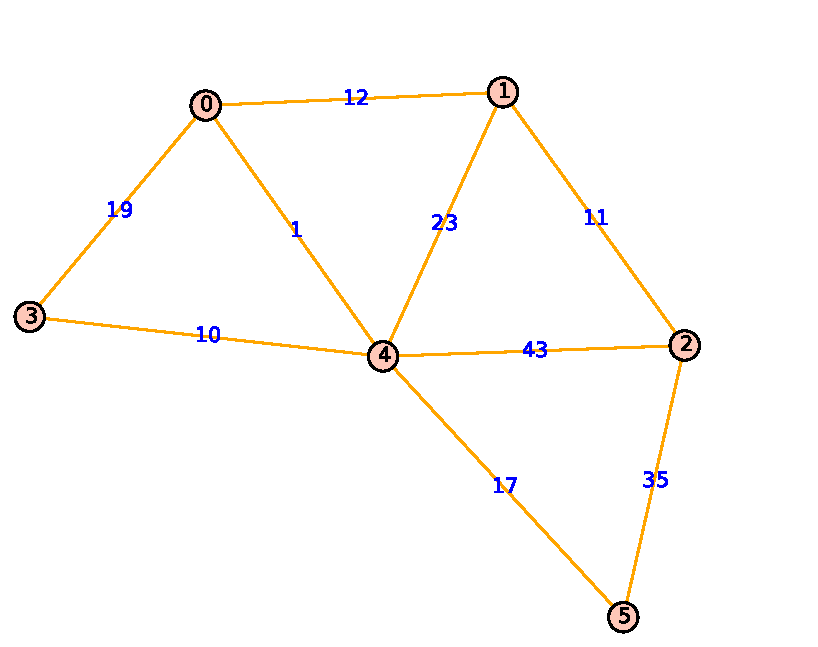
\includegraphics[width=0.35\textwidth]{Weighted_Graph1.pdf}
\caption{\label{fig:Weighted_Graph}This is a weighted graph where the circles represent the nodes; the straight lines represent edges and the numbers on the line represent weights.}
\end{figure}

The Dijkstra's algorithm can be applied to Figure \ref{fig:Weighted_Graph} so that the shortest path from a specific node to any other node can be found.

\section{Basic implementation of Dijkstra's Algorithm}

\subsection{Using Sage}
Using Sage to apply the Dijkstra's Algorithm to a graph is very simple as it has an inbuilt Dijkstra's Algorithm function which can be used to find the shortest path of a graph and the length of the shortest path. In the following link there are two examples; in the first example I have coded accordingly to apply the algorithm on a Weighted graph, and in the second it is applied on a Directed Weighted graph:
\url{https://cloud.sagemath.com/projects/10c09f5d-2e5a-4e24-9208-ea54c7013c14/files/Graphs.sagews}

\begin{figure}[ht]
\centering
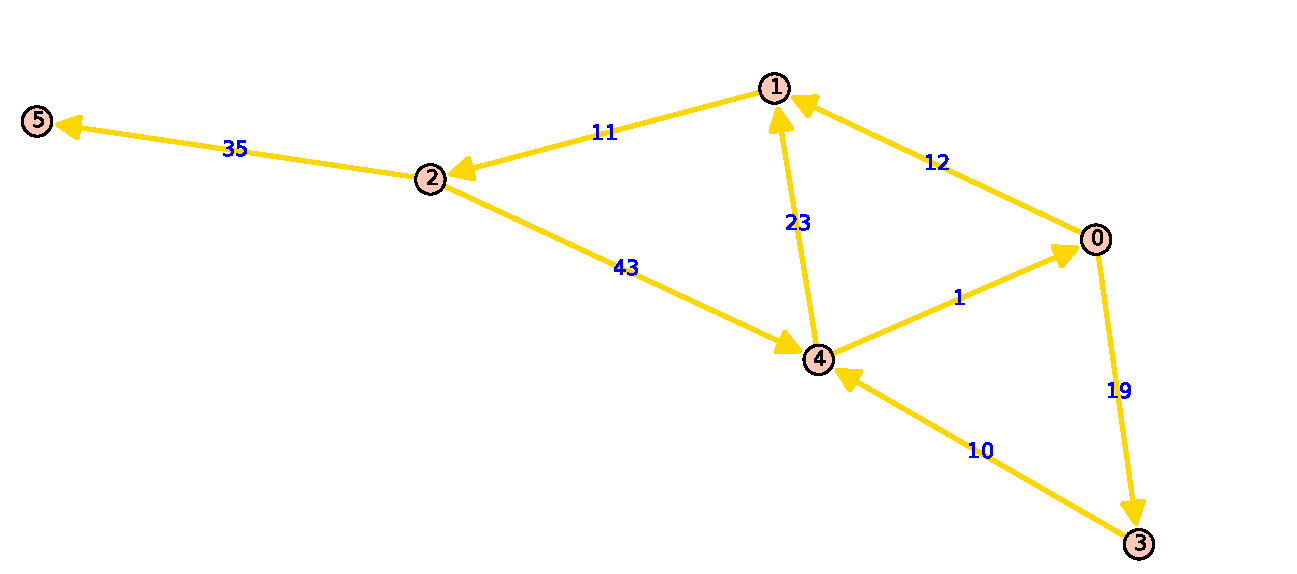
\includegraphics[width=0.5\textwidth,]{DiGraph1.pdf}
\caption{\label{fig:DiGraph}This is a directed graph using the same nodes and weights as represented in Figure \ref{fig:Weighted_Graph}, however the edges are directed.}
\end{figure}

\subsection{Using Python}
Unlike Sage, Python does not have an inbuilt function that can apply the Dijkstra's Algorithm to a network, therefore I had to write a code which specified exactly how the algorithm works. The following is the function I defined which outputs the route of the shortest path:
\begin{verbatim}
def shortest_path(graph, start_vertex, goal_node):
    distances, paths = dijkstra(graph, start_vertex)
    route = [goal_node]
    while goal_node != start_vertex:
        route.append(paths[goal_node])
        goal_node = paths[goal_node]
    route.reverse()
    return route
\end{verbatim}
The full code of the algorithm with comments can be found in: \url{https://cloud.sagemath.com/projects/62875e72-c91c-41e8-812f-c161e5bba8a4/files/Dijkstra's%20Algorithm%20Python1%20.html}. 
\\ Figure \ref{fig:figure 3} is a visualisation of the graph which was used as an example in the code.

\begin{figure}[ht]
\centering
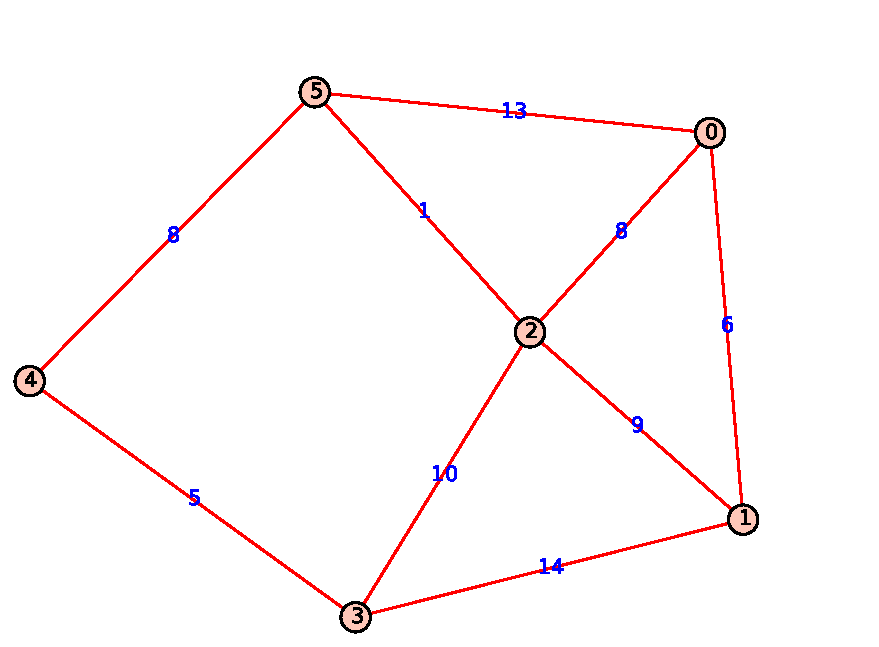
\includegraphics[width=0.4\textwidth]{weighted_python_graph111.pdf}
\caption{\label{fig:figure 3}This is a weighted graph with $6$ nodes, $9$ edges and a total weight of $74$ units.}
\end{figure}

\section{Proof of Correctness}
To prove Dijkstra's Algorithm we have to show: 

$$d(x) = \delta(x) \ \forall x \in R,$$

where $d(x)$ is the path the algorithm computes and $\delta(x)$ is the true shortest path between two nodes $s$ and $x$.

\subsection{By Induction}

 \begin{description}
\item[Base step] $|R| = 1$ and $d(s) = \delta(s) = 0$ is correct.
\item[Inductive Hypothesis] Let $u$ be the last node added to $R$ and $R' = R \cup \{u\}$, then $\forall x \in R' \ d(x) = \delta(x)$. Therefore, for every node in $R'$ that is not $u$, we have the shortest path by the inductive hypothesis. Now, we need to show $d(u) = \delta(u).$
\end{description}
Take $Q$ to have the shortest path $s$ to $u$ for contradiction and has length: 
$$l(Q) < d(u).$$
Assign $xy$ to be the first edge of the path $Q$ that leaves $R'$ and let $q$ be the subpath $s$ to $x$, then:
$$l(q) + l(xy) \leq l(Q).$$
Since $d(x) \leq l(q)$ by inductive hypothesis, we get:
$$d(x) + l(xy) \leq l(q).$$
Node $y$ is adjacent to $x$ and must be updated by the algorithm:
$$d(y) \leq d(x) + l(xy).$$
Since $u$ was picked by the algorithm, $u$ must have the smallest distance computed by the algorithm:
$$d(u) \leq d(y).$$
We can now see when these inequalities are combined the contradiction $d(x) < d(x)$ is formed $\therefore d(u) = \delta(u)$; $Q$ cannot be the shortest path. \cite{Proof}

\bibliographystyle{plain}
\bibliography{Proof_of_Correctness.bib}
\end{document}